\documentclass{article}
\usepackage{graphicx}
\usepackage{wrapfig}
\usepackage{subcaption}
\usepackage[margin=1in]{geometry}
\usepackage{amsmath} % or simply amstext
\usepackage{amssymb}
\usepackage{siunitx}
\usepackage{booktabs}
\usepackage[export]{adjustbox}
\newcommand{\angstrom}{\textup{\AA}}
\newcommand{\colormap}{jet}  % colorbar to use
\usepackage{cleveref}
\usepackage{booktabs}
\usepackage{gensymb}
\usepackage{float}

%BJC: potential titles (uncommented is current favorite)
%\title{The Transport Mechanisms of Polar Solutes in a Cross-linked H\textsubscript{II} Phase Lyotropic Liquid Crystal Membrane}
\title{Size, Shape and Functionality Dependence of Solute Transport Mechanisms in a Cross-linked H\textsubscript{II} Phase Lyotropic Liquid Crystal Membrane}
\author{Benjamin J. Coscia \and Michael R. Shirts} 

\begin{document}

  \graphicspath{{./figures/}}
  \maketitle

  \section{Introduction}

  We need highly selective membranes in order to perform efficient separations.

  H\textsubscript{II} phase lyotropic liquid crystals have densely packed, uniform
  sized pores and have the potential to disrupt conventional membrane separation
  techniques by being selective based not only on size and charge, but on chemical
  functionality as well.

  We can only learn so much from experiment. MD can give us mechanistic insights with
  atomistic resolution so that we can intelligently design new membranes for 
  solute-specific separations.

  In previous work, we determined the most likely structure of the hexagonal phase 
  formed by the monomer Na-GA3C11.
  \begin{itemize}
  	\item We developed techniques for equilibrating the hexagonal phase made by
	neat monomer as well as with varying amounts of water in the pores.
  \end{itemize} 

  In this work, we have determined the transport mechanisms and macroscopic
  transport properties exhibited by a number of polar solutes with varying size,
  chemical functionality and hydrophilic character.
  \begin{itemize}
	\item Many of the separations we are interested in involve polar organic 
	compounds.
  \end{itemize} 

  We have compared our calculated diffusion coefficients with experimental
  measurements made using DOSY NMR. 

  \section{Methods}

  \subsection{Molecular Dynamics Simulations}
  
  \subsubsection*{System Setup}

  Stable H\textsubscript{II} phases, assembled with Na-GA3C11, can be formed
  using a broad range of water concentrations.
  \begin{itemize}
	\item In the literature, this system is typically synthesized with close
	to 10 wt \% water \cite{smith_ordered_1997, zhou_new_2007}
    \item However, Resel et al. noted that the system is likely fully 
	hydrated with less than 7 wt \% water. \cite{resel_h2-phase_2000}
	\item We decided to test two different levels of water content: 5 and 10 wt \%
  \end{itemize} 

  We observed that water partitions into the tail region of our system and therefore
  built our initial configurations with water in both regions close to the expected
  equilibrium value.
  \begin{itemize}
	\item There is about 2:1 water in the pores versus in the tails for the 10 wt \% system.
	\item The amount of water present in the tails may or may not be experimentally consistent
	but if we don't put it in, the results will not be thermodynamically consistent, which 
	will give issues with measurements and calculations.
	\item See supporting info for water equilibration simulation data.
	\item We adjusted the pore radius in our systems so that the right amount of water
	fits in the pores without any vacuum using \texttt{gmx solvate}.
	\item We placed water molecules in the tail region one at a time in random locations
	with short energy minimizations between insertions.
  \end{itemize}

%  We equilibrated the initial configuration using the `wet' equilibration procedure
%  described in our previous work (reference to structure paper).
  %BJC: not sure I need to go into any details describing that procedure
%  \begin{itemize}
%	\item Series of NVT simulations with force constants on carbon atoms of aromatic
%	ring in head group
%	\item Force constants reduced according to the sequence: 1000000, 3162,
%	56, 8, 3, 2, 1, 0 kJ mol$^{-1}$ nm$^{-2}$ 
%  \end{itemize}

%  We cross-linked the equilibrated solvated configuration using the cross-linking procedure
%  described in our previous work. 

  We equilibrated an initial solvated configuration before adding solutes.
  \begin{itemize}
	\item We equilibrated the initial configuration using the `wet'
	equilibration procedure described in our previous work~\cite{coscia_understanding_2019}.
	\item We cross-linked the equilibrated solvated configuration using the
	cross-linking procedure described in our previous work. 
  \end{itemize}

  We added 6 solute molecules to each pore of the equilibrated cross-linked
  configuration.
  \begin{itemize}
	\item We equally spaced each solute in the pore
	\item 6 solutes per pore provided a balance of a useful amount of data
	for generating statistics and a low degree of interaction between solutes (reference
	to supporting information to show low degree of interaction)
	\item At each insertion point we placed a randomly oriented solute molecule
	then ran a short energy minimization.
	\item We allowed the solutes to equilibrate for 5 ns using berendsen 
	pressure control
	\item We collected transport data using 1 $\mu$s simulations
  \end{itemize}
  
%  \subsubsection*{Modeling subdiffusion}\label{method:model_sFBM}
%
%  Solutes in our H\textsubscript{II} LLC membrane exhibit subdiffusive
%  behavior, a type of anomalous diffusion. 
%  \begin{itemize}
%  	\item During an anomalous diffusion process, the mean squared displacement (MSD)
%  	does not grow linearly with time, rather it is of the form:
%	\begin{equation} 
%	\langle x^2(t) \rangle = K_{\alpha}t^\alpha
%	\label{eqn:msd_form}
%	\end{equation} 
%	where $\alpha$ is the anomalous exponent and $K_\alpha$ is the
%	generalized diffusion coefficient.
%	\item A value of $\alpha < 1$ indicates a subdiffusive process, while a value of
%	$\alpha = 1$ and $\alpha > 0$ is characteristic of Brownian and superdiffusive
%	motion respectively.
%  \end{itemize}
%
%  \noindent We calculated both the ensemble-averaged and time-averaged MSDs
%  of the simulated trajectories.
%  \begin{itemize}
%	\item The ensemble-averaged MSD measures the displacement of a particle from its initial
%	position~\cite{meroz_toolbox_2015} and can be written as
%	\begin{equation}
%	\langle x^2(t) \rangle = \langle x(t) - x(0) \rangle
%	\label{eqn:ensemble_msd}
%	\end{equation}
%%	\item The average MSD calculated in this way recovers the form of
%%	Equation~\ref{eqn:msd_form}. % time-averaged should recover it too for FBM 
%	\item The time-averaged MSD measures the displacement between all possible time lags
%	and can be written as
%	\begin{equation}
%	\overline{x^2(\tau)} = \dfrac{1}{T - \tau}\int_{0}^{T - \tau} (x(t + \tau) - x(t))^2 dt
%	\end{equation}
%	where $\tau$ is the time lag and T is the length of the
%	trajectory~\cite{meroz_toolbox_2015}. 
%%	\item The time-averaged MSD becomes linear in our simulations,
%%	therefore we can fit a line to its slope in order to estimate the macroscopic
%%	diffusivity of the particle.
%	%BJC: this needs more justification. Not many people have done it
%	%BJC: could also not report them as diffusivities. Comparison of total MSD
%	% should give same information
%	% Linear region probably exists because dwell times on the order of large lag times
%	% become negligible
%  \end{itemize}
%  
%  \noindent Three common mathematical models for modeling anomalous subdiffusion processes include 
%  continuous time random walks (CTRW), fractional Brownian motion (FBM) and
%  random walks on fractals (RWF).\cite{meroz_toolbox_2015}
%  \begin{itemize}
%    \item FBM is common in crowded, viscoelastic environments where each step comes 
%    from a Gaussian distribution but is anti-correlated to its previous 
%    step.~\cite{mandelbrot_fractional_1968,jeon_fractional_2010,banks_anomalous_2005}
%    \item A CTRW is characterized by a distribution of hop lengths and 
%    dwell times, where each each step is characterized by independent random draws from 
%    each distribution.\cite{montroll_random_1965,morrin_three_2018}
%    \item An RWF is imposed by a system's geometry. Systems with tortuous pathways and dead
%    ends cause anti-correlated motion.\cite{meroz_toolbox_2015,neusius_subdiffusion_2008}
%    \item The processes described above can happen alone or in combination.  	
%  \end{itemize}
%  
%  \noindent We believe that solutes in the system studied here exhibit subordinated 
%  fractional Brownian motion (sFBM) where the parent process is FBM and the 
%  leading process is a CTRW. 
%  \begin{itemize}
%  	\item The ensemble-averaged MSD differs from the time-averaged MSD, which
%  	is indicative of non-ergodicity, a trait inherent to CTRWs but not FBM or RWFs.~\cite{thiel_weak_2014}
%  	\item We also observe non-stationary $z$-coordinate traces of each solute's
%  	center of mass (COM). %BJC: figure of a z-coordinate trace in main text or in supporting info
%  	\item For a pure CTRW, the time-averaged MSD should be linear.
%  	~\cite{neusius_subdiffusion_2008,meroz_subdiffusion_2010}
%  	\item However, a typical time-averaged solute MSD is sublinear (see supporting
%  	information), which suggests that there is another underlying subdiffusive mechanism.
%  	\item The hop lengths recorded after each dwell period are anti-correlated (See supporting information)
%  	\item Given the viscoelastic nature of the monomers in our system, we believe
%  	the hop lengths can be modeled with FBM. 
% 	\item For subordinated FBM, it can be shown that
%  	\begin{equation}
%  	\langle x^2(t) \rangle \simeq t^{\alpha\beta}
%  	\end{equation}
%  	where $\alpha$ is the anomalous exponent characteristic of the leading CTRW process
%  	and $\beta$ is the anomalous exponent characteristic of the parent FBM process. 
%  \end{itemize}
%
%  \noindent We can characterize a CTRW process using the parameters which describe its
%  dwell time and hop length distribution.
%  \begin{itemize}
%	\item We used the \texttt{ruptures} python package in order to identify
%	breakpoints in solute trajectories.\cite{truong_ruptures:_2018} (See Supporting Information for more
%	details on chosen parameters. i.e. type of cost function, cost function penalty
%	tolerance, number of dimensions used)
%	\item The corresponding hop lengths and dwell times between break points were 
%	used to construct empirical distributions.
%	\item For solutes in our system, the distribution of hop lengths is
%	well-represented by a Gaussian distribution.~\cite{metzler_random_2000,
%	metzler_anomalous_2014,neusius_subdiffusion_2009}
%	\item We are most interested in the standard deviation, $\sigma$, of the 
%	hop length distribution.
%	\item The distribution of dwell	times is expected to fit a power law (or heavy-tailed)
%	distribution proportional to $t^{-1-\alpha}$.~\cite{meroz_toolbox_2015}
%	\item Because we are limited to taking measurements at discrete values
%	dictated by the output frequency of our simulation trajectories, we fit the
%	empirical dwell times to a discrete power law distribution whose maximum
%	likelihood $\alpha$ parameter we calculated by maximizing the following
%	likelihood function: 
%        \begin{equation}
%	\mathcal{L}(\beta) = -n\text{ln}\zeta(\beta, x_{min}) -
%	\beta\sum_{i=1}^{n} \text{ln}~x_i 
%	\label{eqn:powerlaw_likelihood}
%	\end{equation}
%	where $\beta = 1 + \alpha$, $x_i$ are collected dwell time data points,
%	$n$ the total number of data points, and $\zeta$ is the Hurwitz zeta function
%	where $x_{min}$ is the smallest measured value of
%	$x_i$.~\cite{clauset_power-law_2009} 
%	\item We obtained distributions of the hop length standard deviations, $\sigma$, and
%	$\alpha$ using statistical bootstrapping.\cite{efron_introduction_1994} 
%  \end{itemize}
%  
%  \noindent FBM processes can be described using the Hurst parameter, $H$, where 
%  $H = \beta/2$.
%  \begin{itemize}
%  	\item Brownian motion is recovered for $H = 0.5$
%	\item The autocovariance function of hop lengths has the analytical form:~\cite{mandelbrot_fractional_1968}
%    \begin{equation}
%	\gamma(k) = \dfrac{1}{2}\bigg[|k-1|^{2H} - 2|k|^{2H} + |k+1|^{2H}\bigg]
%	\label{eqn:autocovariance}
%	\end{equation}
%	where $k$ is the number of increments between hops.
%	\item We obtained H by performing a least squares fit of Equation~\ref{eqn:autocovariance}
%	to the empirically measured autocovariance function.
%	\item We used statistical bootstrapping to generate a distribution of $H$ 
%	values. %BJC: can provide more detail in supporting or just reference python script
%  \end{itemize}
%
%%  We generated distributions of parameters for the dwell time and hop length
%%  distributions using statistical bootstrapping.
%%  \begin{itemize}
%%	\item For each type of distribution, we randomly selected $n$ data points from the empirical
%%	distribution with replacement.
%%	\item We repeated the fitting procedure described above for each of 200 bootstrap trials.
%%  \end{itemize} 
%
%%  We calculated macroscopic diffusion coefficients by simulating trajectories orders of
%%  magnitude longer than our molecular simulations.
%  \noindent For each solute, we simulated 10000 sFBM trajectories for 1 $\mu$s each. 
%  \begin{itemize}
%	\item We constructed trajectories by simulating	sequences of dwell times and correlated 
%	hop	lengths generated based on parameters randomly chosen from our bootstrapped parameter
%	distributions.
%	\item We propagated each trajectory until the total time reached 1 $\mu$s, and truncated
%	the last data point so that the total time exactly equaled 1 $\mu$s. 
%    \item Valid comparisons are only possible between fixed length sFBM simulations. The
%    power law dwell time behavior gives rise to the aging phenomenon, embodied by
%    a decrease in MSD with measurement time.~\cite{neusius_subdiffusion_2008,metzler_anomalous_2014}
%    \item We reported the MSD after 1 $\mu$s with corresponding 95 \% intervals
%% Following probably better suited for supporting information, if included at all
%%	\item We randomly sample Gaussian hop lengths using the
%%	\texttt{numpy.random.normal} method of the \texttt{numpy} python package.
%%	\item We randomly sampled dwell times from a discrete power law
%%	distribution based on the recommendations of Clauset et
%%	al.~\cite{clauset_power-law_2009}: 
%%	\begin{equation}
%%	x = \lfloor
%%	(x_{min} - \tfrac{1}{2})(1 - r)^{-1/(\alpha - 1)} + \tfrac{1}{2} \rfloor
%%	\label{eqn:discrete_powerlaw_draws}
%%	\end{equation}
%%	where $r$ is randomly drawn from a uniform distribution which we simulated
%%	with \texttt{numpy.random.uniform}.
%%	\item We found that thermal noise does not significantly influence the MSD and
%%	therefore did not add any noise to the simulated trajectories. (See supporting info)
%  \end{itemize}
%
%%BJC: probably don't need to explain this in great detail
%%  \noindent We fixed the length of each simulated trajectory so that we could compare the total
%%  MSD between different solutes without the influence of the ageing phenomenon.
%%  \begin{itemize}
%%	\item Ageing is defined by the tendency of the average MSD to decrease
%%	as the length of trajectories are increased~\cite{metzler_anomalous_2014}.
%%	\item The maximum measured dwell time can be no longer than the total length
%%	of a simulated trajectory. 
%%	\item As measurement time or trajectory length is increased, longer dwell times
%%	are incorporated into the calculation, lowering the average MSD. (See supporting
%%	info for demonstration)
%%	\item We can achieve consistent total MSDs with low uncertainty for
%%	simulated trajectories created with a given set of parameters if we fix the
%%	trajectory length (as opposed to total number of steps).  
%%  \end{itemize}

  \subsubsection*{Radial Distribution Functions}

  We measured the average radial distance of each solute of interest from the pore
  centers.
  \begin{itemize}
	\item We binned the radial distances and then normalized by the volume
	of the annulus defined by the bin edges.
	\item Although the pores are often described as straight, they have a
	small degree of tortuosity which disrupts the RDF calcuation 
	\item We obtain the best RDF by constructing splines that run through the
	pore centers.
	\item We construct the splines by dividing the membrane into 20 slices
	in the $z$-direction. Within each slice, we calculate the location of 
	the pore centers based on the average location of the aromatic rings
	that make up the monomer head groups.
	\item When calculating the RDF, the radial distance from the pore center
	is based on the distance between the solute center-of-mass and the ($x$, $y$)
	coordinates of appropriate point on the spline.
  \end{itemize}

  \subsubsection*{Coordination number}

  We quantified the coordination of solutes with surrounding molecules.
  \begin{itemize}
  	\item For each frame, we counted the identities and number of
  	coordinated molecules to a given solute based on a distance cut-off. 
	\item We found that this approach is more useful than calculating the
	3D spherical radial distribution function because it gives detailed
	frame-by-frame information rather than an average. 
  \end{itemize}
   
  \section{Results and Discussion}
  
  \subsection*{Governing Mechanisms}\label{section:mechanism_overview}  
  
  % BJC: seems right to summarize overarching mechanisms observed first  
  On the timescales simulated in our study, solutes exhibit subdiffusive
  transport behavior as evidenced by their sublinear MSD curves. 
  \begin{itemize}  
	\item As an example, the MSD curve for ethanol is plotted in 
	Figure~\ref{fig:example_msd}.
  \end{itemize}
  
  \noindent All solutes exhibit hop diffusion, characteristic of a continuous time random walk.
  \begin{itemize}
  	\item Figure~\ref{fig:example_ztraces} shows the $z$-coordinate versus time of
  	3 representative ethanol centers of mass.
  	\item There are clear periods of entrapment separated by relatively large hops.
  	\item The length of entrapment follows a power law distribution 
  	(Figure~\ref{fig:example_powerlaw}) and the distribution of hop lengths can be 
  	described with a Gaussian distribution (Figure~\ref{fig:example_hop_dist}).
  	\item Power law distributed dwell times are responsible for the ageing phenomenon
  	which causes the MSD curve to decrease with increasing measurement time as longer
  	dwell times get sampled.
  \end{itemize}
  
  \noindent The direction of each hop is anti-correlated to the direction of the previous hop.
  \begin{itemize}
  	\item Figure~\ref{fig:example_autocovariance} shows the autocovariance function of 
  	ethanol step vectors. % BJC: vectors because includes magnitude + direction. Better word?
  	\item The negative autocovariance at low values of k indicates anti-correlation
  	between steps. 
  	\item If solutes followed a pure CTRW mechanism, the autocovariance function would
  	decay to zero immediately.
  	\item Although the autocovariance function is relatively noise, due to the somewhat small
  	number of hops observed over the course of each solute trajectory, there is the least 
  	uncertainty at k=1, the most insightful data point. This behavior is consistent across
  	all solutes molecules.
  	\item Therefore, we believe transport can be described as subordinated fractional Brownian
  	motion where the leading process is a CTRW with hops that are dictated by the parent
  	process, FBM.
  	\item Future publications will focus on modeling the solute's transport characteristics
  	with an sFBM model
  \end{itemize}

% BJC: first iteration of figure after this before I decided to include a hop length and dwell time distribution
%  \begin{figure}
%  \centering
%  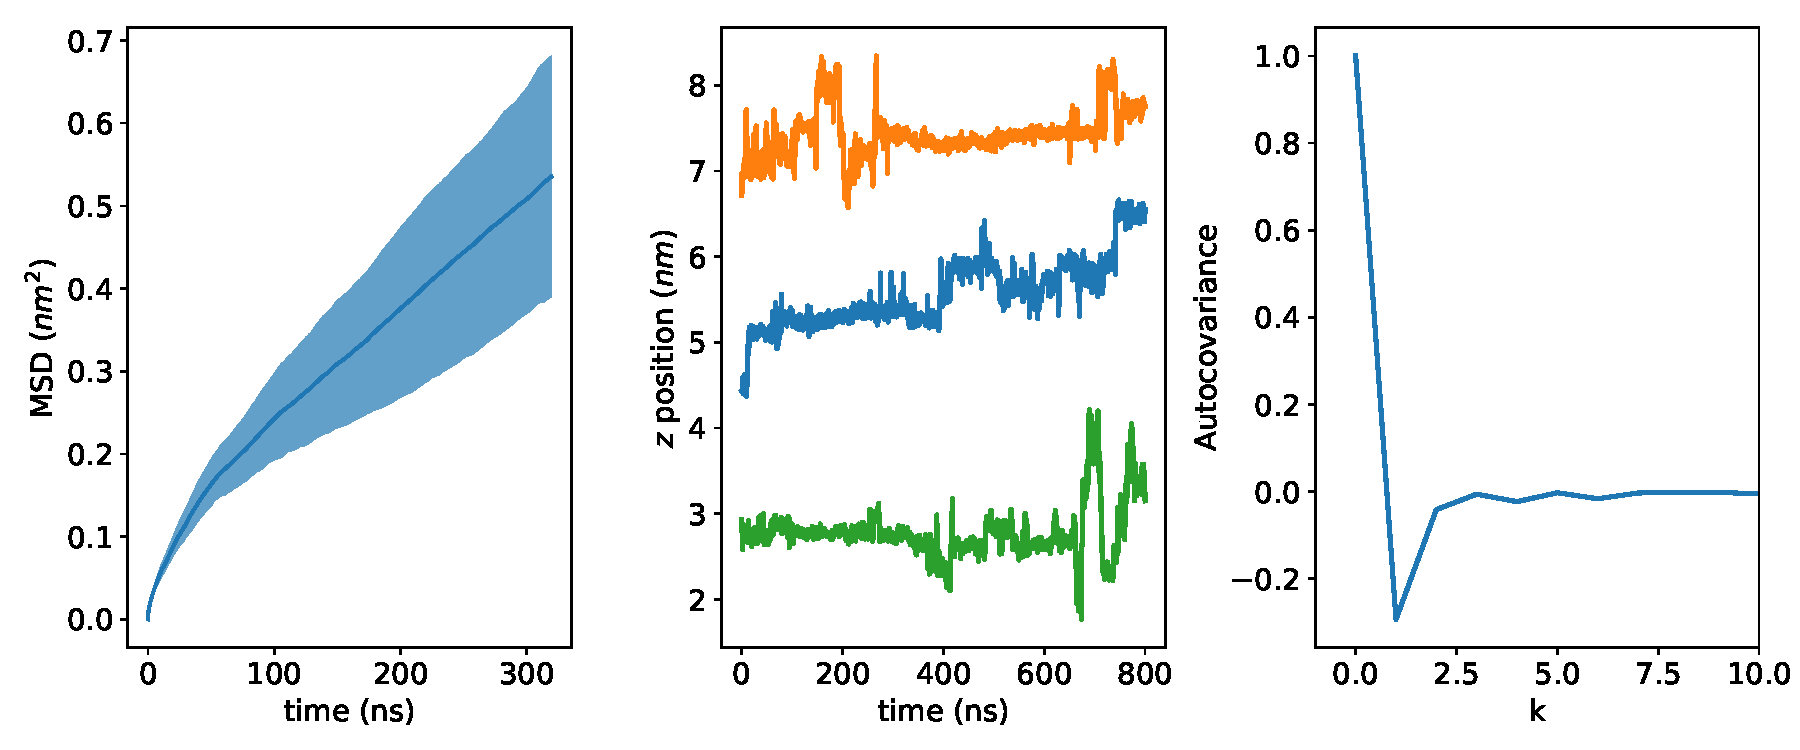
\includegraphics[width=\textwidth]{msd_ztrace_acf.pdf}
%  \caption{}\label{fig:msd_ztrace_acf}
%  \end{figure}

  \begin{figure}
  \centering
  \begin{subfigure}{0.49\textwidth}
  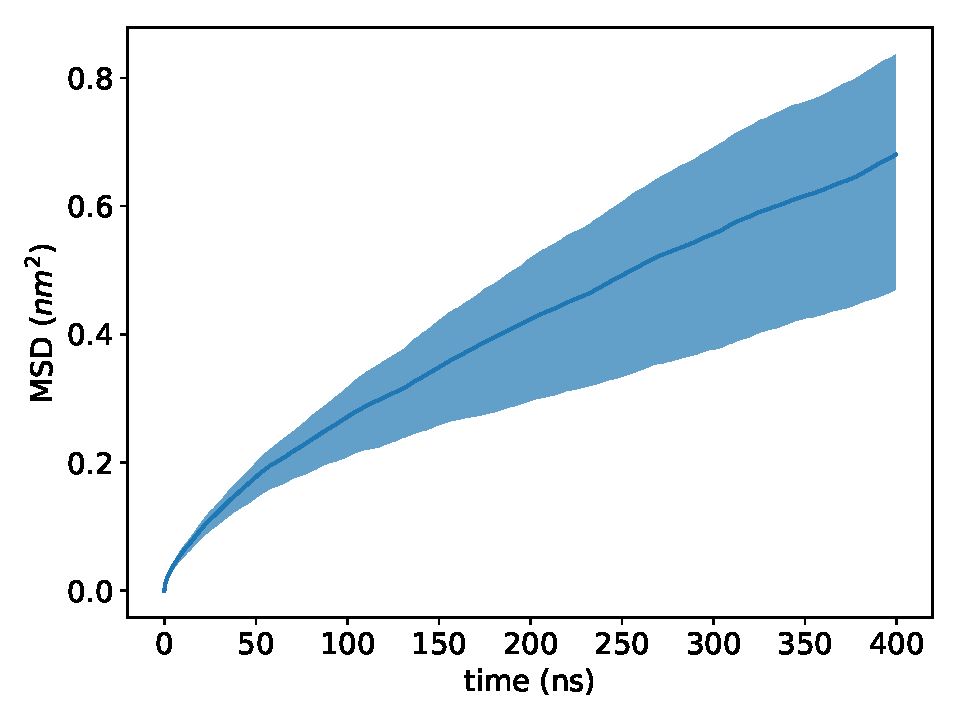
\includegraphics[width=\linewidth]{example_msd.pdf}
  \caption{}\label{fig:example_msd}
  \end{subfigure}
  \begin{subfigure}{0.49\textwidth}
  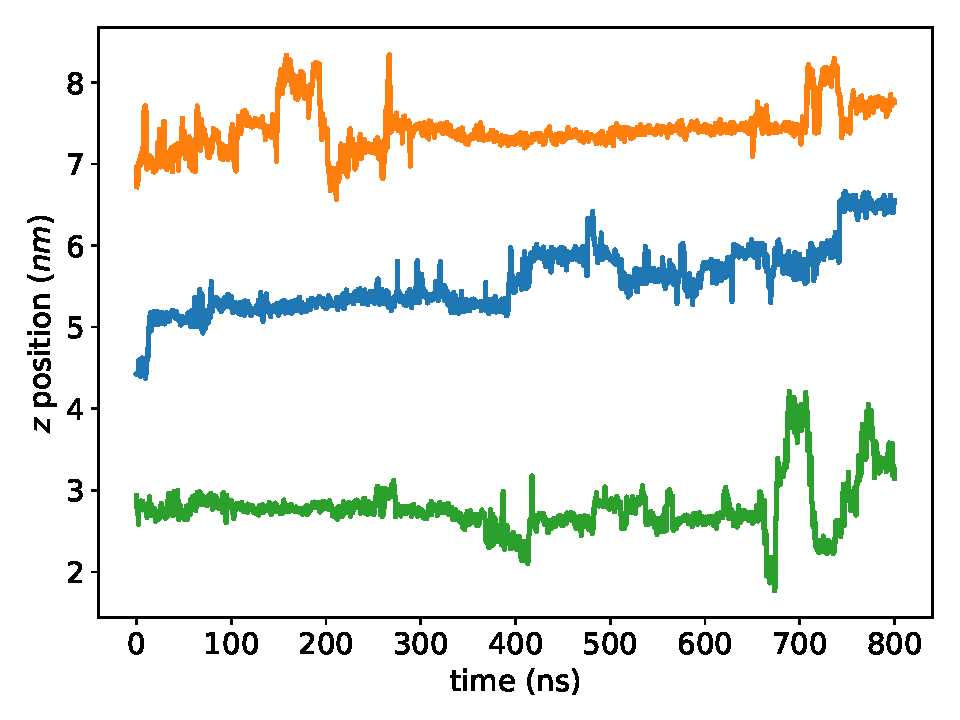
\includegraphics[width=\linewidth]{example_ztraces.pdf}
  \caption{}\label{fig:example_ztraces}
  \end{subfigure}
  \par\medskip
  \begin{subfigure}{0.325\textwidth}
  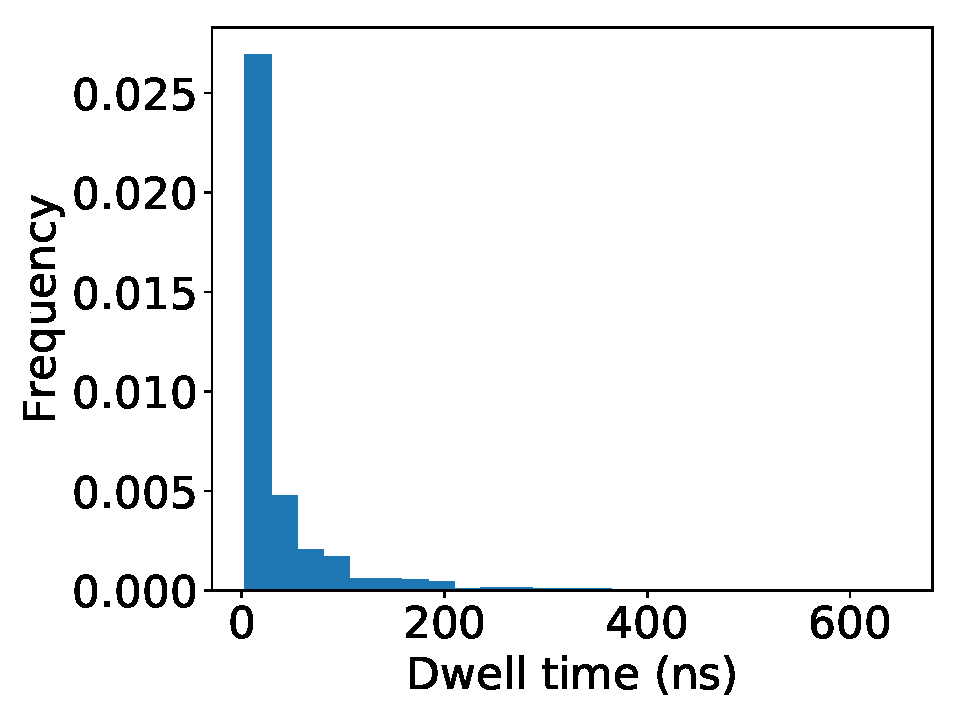
\includegraphics[width=\linewidth]{example_powerlaw.pdf}
  \caption{}\label{fig:example_powerlaw}
  \end{subfigure}
  \begin{subfigure}{0.325\textwidth}
  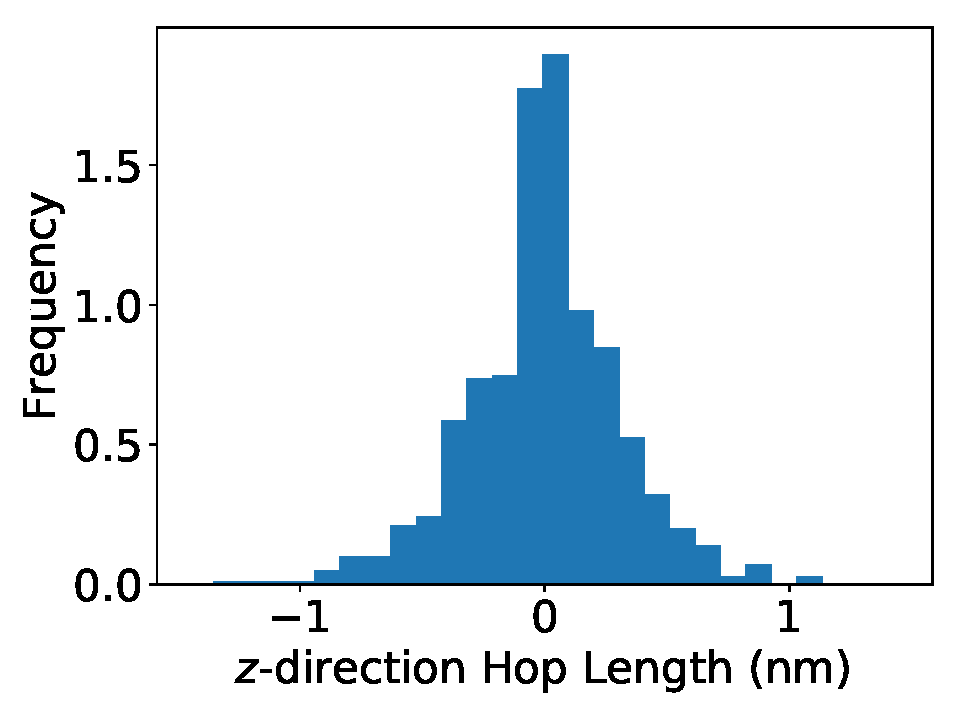
\includegraphics[width=\linewidth]{example_hop_dist.pdf}
  \caption{}\label{fig:example_hop_dist}
  \end{subfigure}
  \begin{subfigure}{0.325\textwidth}
  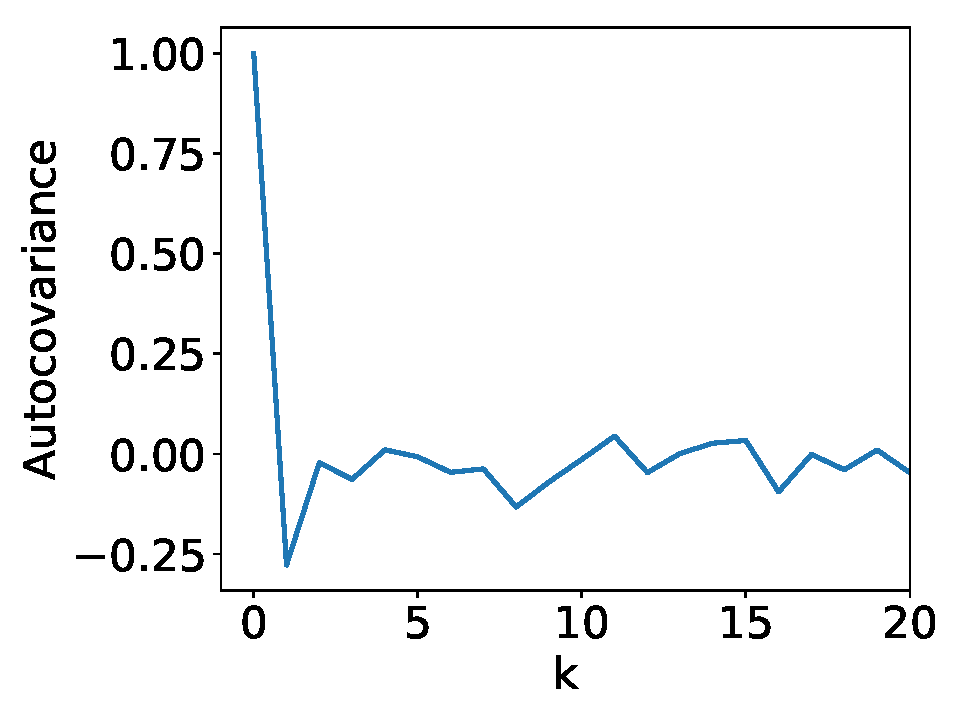
\includegraphics[width=\linewidth]{example_autocovariance.pdf}
  \caption{}\label{fig:example_autocovariance}
  \end{subfigure}
  \caption{All solutes show subdiffusive transport behavior inside the membrane's
  nanopores, similar to that exhibited by ethanol. (a) The time-averaged MSD of 
  ethanol is not linear which suggests transport is governed by an anomalous 
  subdiffusion process. (b) The $z$-coordinate trace of 3 representative ethanol
  COMs shows clear periods of entrapment separated by hops. (c) The distribution
  of dwell times follows a power law. (d) The distribution of hop lengths appears
  Gaussian. (e) Hops are anti-correlated to their previous hop as indicated by the
  negative value of the autocovariance function at $k$ = 1.}\label{fig:examples}
  \end{figure}
  
  % BJC: would it be better to report as a fraction of water MSD?
  % BJC: need MSDs of 5 wt % systems here too. Can narrow to study of 10 wt % systems after
  \noindent We calculated the time-averaged MSD of each solute in the set over the
  course of 1 $\mu$s MD simulations. 
  \begin{itemize}
    \item Because the MSDs are non-linear and because of the ageing phenomenon, we
    did not attempt to calculate a diffusion constant as one might for a Brownian
    particle with a linear MSD.
	\item Instead, the MSD values plotted in Figure~\ref{fig:all_msds} represent the
	average MSD of each solute after a 400 ns time lag.
  \end{itemize}  
  
%  \subsubsection*{The Influence of Water Content on Macroscopic Diffusion Coefficients}
%
%  Solutes in systems with lower water content exhibit lower diffusion coefficients.
%  \begin{itemize}
%	\item Pores are more crowded when there is less water (show RDFs of each)
%	\item Not a linear function of pore size - radius increase by x, D increases by y
%	\item Larger influence on bigger molecules
%  \end{itemize}
  
  \begin{figure}
  \centering
  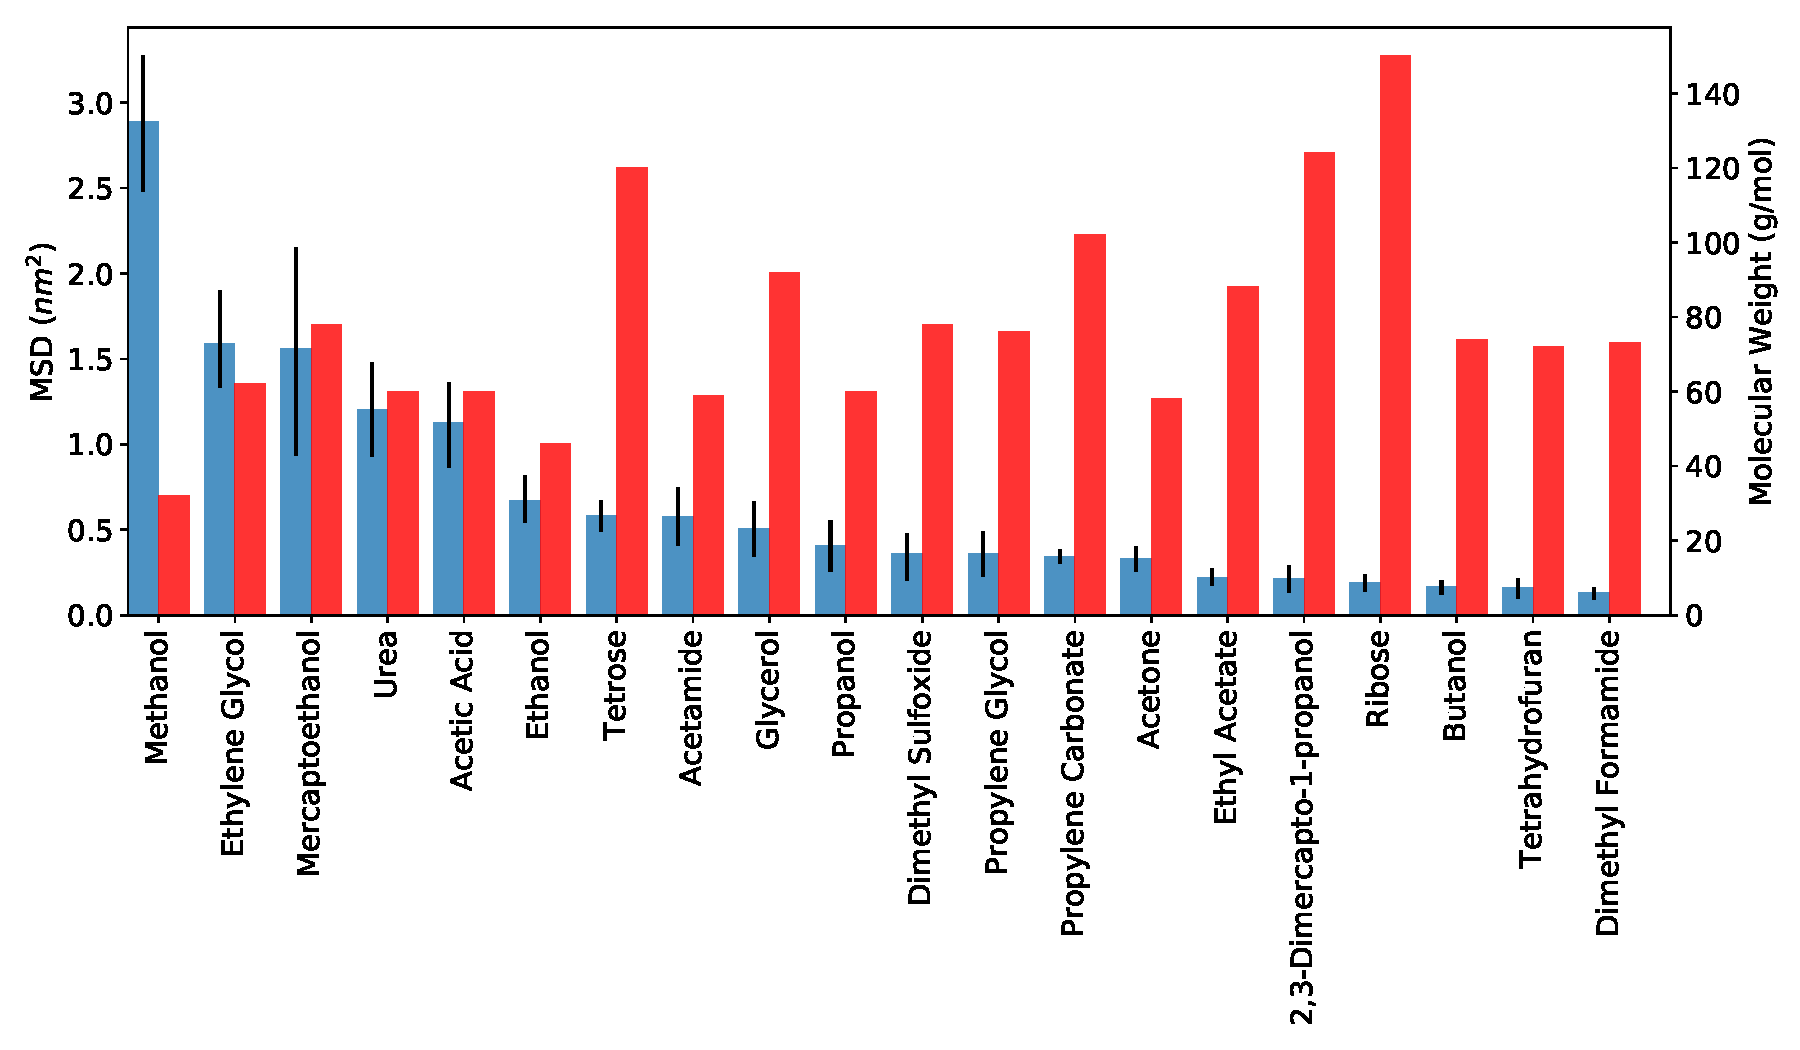
\includegraphics[width=\textwidth]{all_tamsds.pdf}  % include bar plot of MW to show it's non-monotonic
  \caption{}\label{fig:all_msds}
  \end{figure}
  
  \noindent The MSDs are not a monotonic function of solute molecular weight.
  \begin{itemize}
  	\item We plotted the solute molecular weights alongside their MSDs in Figure~\ref{fig:all_msds}.
  	\item Transport is clearly affected by factors other than molecular weight. 
  	\item Tetrose, our third heaviest solute, has an MSD higher than more than half of
  	all solutes studied. 
  	\item The three slowest solutes have lower molecular weights than 8 faster solutes.
  \end{itemize}
  
  \noindent The MSDs in Figure~\ref{fig:all_msds} are a strong function of two solute 
  trapping mechanisms. % by which solutes become trapped.
  \begin{itemize}
  	\item Solutes that are hydrogen bond donors can be stabilized through hydrogen bonds
  	with one of the five oxygen atoms attached to each monomer head group. 
  	\item In a separate interaction, solutes can become kinetically trapped between 
  	monomer head groups. These interactions likely lead to the observed anti-correlated
  	hopping	behavior.
  	\item Generally, both mechanisms affect each solute to varying degrees.
  \end{itemize}
  
  %BJC: somewhere need to say why solutes preferentially hbond with carboxylate groups -- is this real
  
  %BJC: This will need updating once all the rest of outline is written.
  \noindent The degree to which solutes are influenced by each entrapment mechanism
  is a complex function of a solute's size, shape, and polarity.
  \begin{itemize}
    \item In general, solutes can move fastest in the pore center, where
    there is comparatively little resistance to diffusion.
	\item The 5 fastest solutes in our study have a low molecular weight and
	spend a significant amount of time in the pore center. They are only slowed
	by hydrogen bonds with monomer carboxylate groups.
	\item Bulky solutes with many hydrogen bond donating groups, like glycerol,
	spend most of their time in the pore center, but their large size combined
	with a higher solute-head group hydrogen bond frequency, makes their dynamics slow. 
    \item Solutes with high hydrophobic character tend to partition into the 
    head group region where entrapment occurs.
    \item We observe low MW solutes with lower-than-expected MSDs because they
    spend more time trapped between monomer head groups due to low water
    solubility.
    \item Small, planar molecules like acetone exhibit some of the slowest MSDs.
    Their flat geometry and small size makes it easy for them to get lodged deep
    between head groups.
  	\item Overall solutes exhibit some degree of trapping, by one or a combination of the above
  	mechanisms, with anticorrelated hops between each period of immobility due to 
  	obstructions.
  \end{itemize}
  
  We will revisit these observations in the the context of specific groups of 
  molecules in the discussion that follows.

%  We will explore these factors in greater detail in the context of 
%  specific groups of molecules in the discussion that follows.

  \subsection*{Transport of Water}

  Water molecules also exhibit hop diffusion.
  
  The overwhelming number of water molecules reduces

  Even in the center of the pore, where the density of water molecules is
  highest, individual water molecules exhibit hop diffusion as they create a
  tight hydrogen bond network.
  %TODO: the following is a hypothesis
  \begin{itemize}
	\item Water sticks to pore walls
	\item Dwell times are short
	\item Water tumbles across pore for a while until it sticks again. 
	\item Water gets caught in h-bonds with other water molecules away
	from pore center.
  \end{itemize}

  In this confined environment, the diffusion constant is x times lower than
  expected bulk diffusion coefficient of tip3p water.

  %TODO: study diffusion mechanism of water
  
  \subsection*{Transport of Simple Alcohols}

  The MSD of methanol, ethanol, propanol and butanol descends in order of 
  their molecular weight, however, methanol travels faster than expected.  %BJC: find approximate relationship between MW and mobility
  \begin{itemize}  
    \item The radial distribution as a function of distance from the pore center
    for each alcohol is plotted in Figure~\ref{fig:simple_alcohol_rdf}.
    \item On average, the density of methanol in the pore center is only slightly
    less than the density near the head groups.
    \item All other alcohol molecules are concentrated in the head group region.
  \end{itemize}
  
  All simple alcohols participate in a similar number of hydrogen bonding interactions
  with the monomer head groups, but with varying preference towards hydrogen bonds with
  the monomer carboxylate oxygen atoms (See Figure~\ref{fig:simple_alcohol_hbonds}).
  \begin{itemize}
  	\item If all 5 hydrogen bonding acceptor sites on the monomer head groups were equal,
  	we would expect the ratio of the number of hydrogen bonds between solutes and the two 
  	carboxylate oxygen atoms to the number of hydrogen bonds between solutes and the three
  	ether groups to be 2/3. 
  	\item There is a clear preference towards hydrogen bonding with the carboxylate 
  	oxygen atoms for all simple alcohols.
  	\item This is largely due to the more highly crowded environment surrounding the ether
  	oxygen atoms.
  	\item Butanol shows the largest preference towards hydrogen bonds with carboxylate 
  	head groups.
  	\item The radial distribution function of atoms located at opposite ends of butanol
  	shows that, on average, oxygen atoms are situated 0.25 nm closer to the pore centers
  	than the distal carbon atoms.
  	\item This suggests that alcohols tend to orient themselves like the liquid crystal 
  	monomers, with hydrophilic components point towards the pore centers.
  \end{itemize}
  
  \begin{figure}
  \centering
  \begin{subfigure}{0.325\textwidth}
  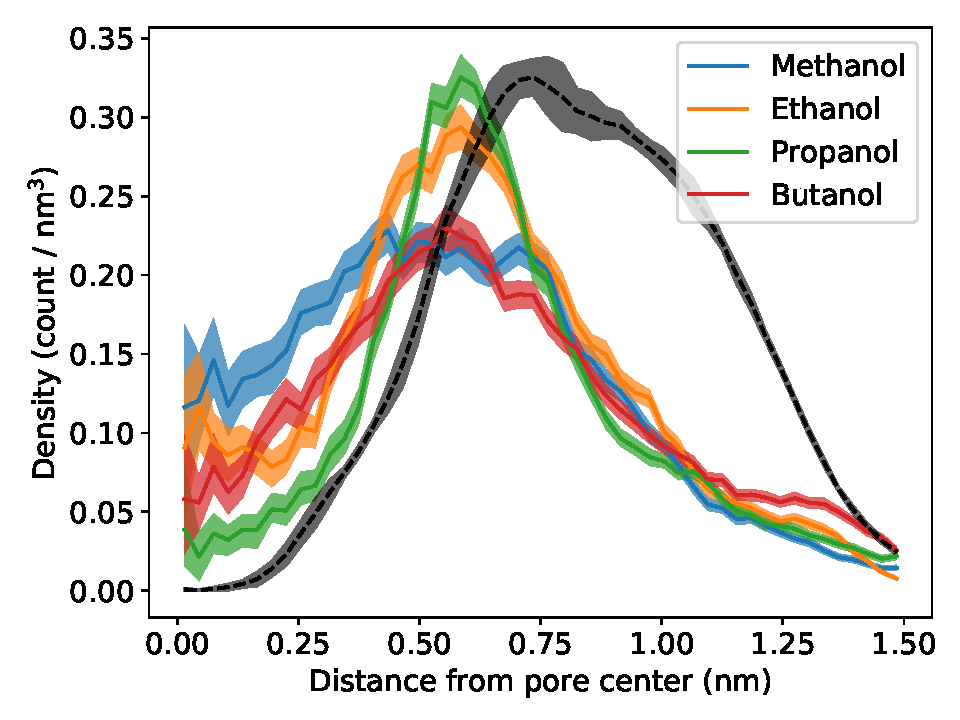
\includegraphics[width=\linewidth]{simple_alcohol_rdf.pdf}
  \caption{}\label{fig:simple_alcohol_rdf}
  \end{subfigure}
  \begin{subfigure}{0.325\textwidth}
  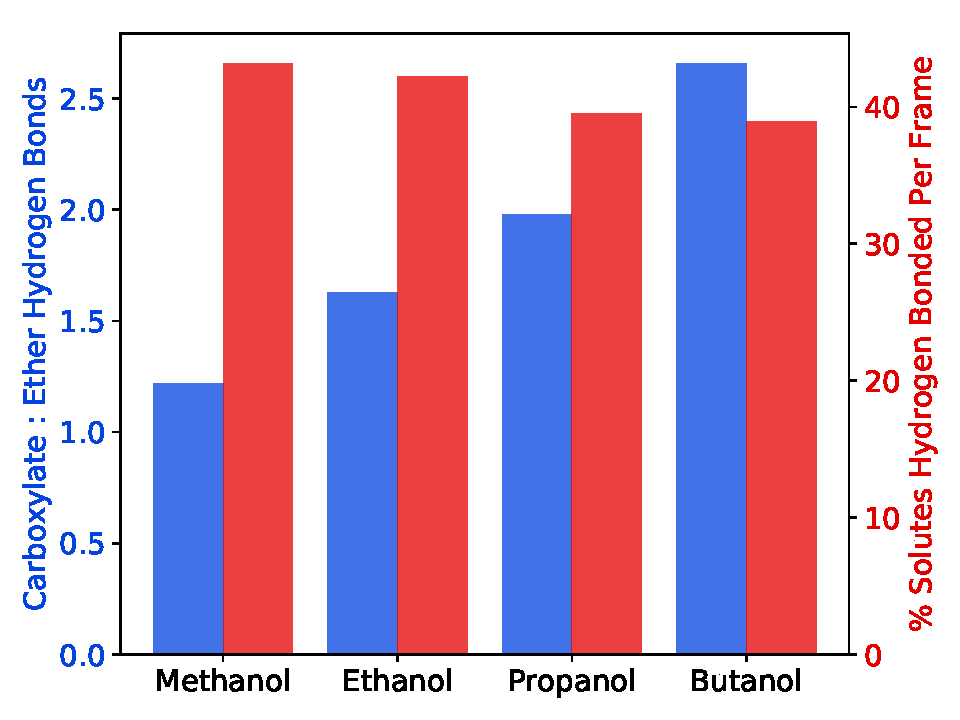
\includegraphics[width=\linewidth]{simple_alcohol_hbonds.pdf}
  \caption{}\label{fig:simple_alcohol_hbonds}
  \end{subfigure}
  \begin{subfigure}{0.325\textwidth}
  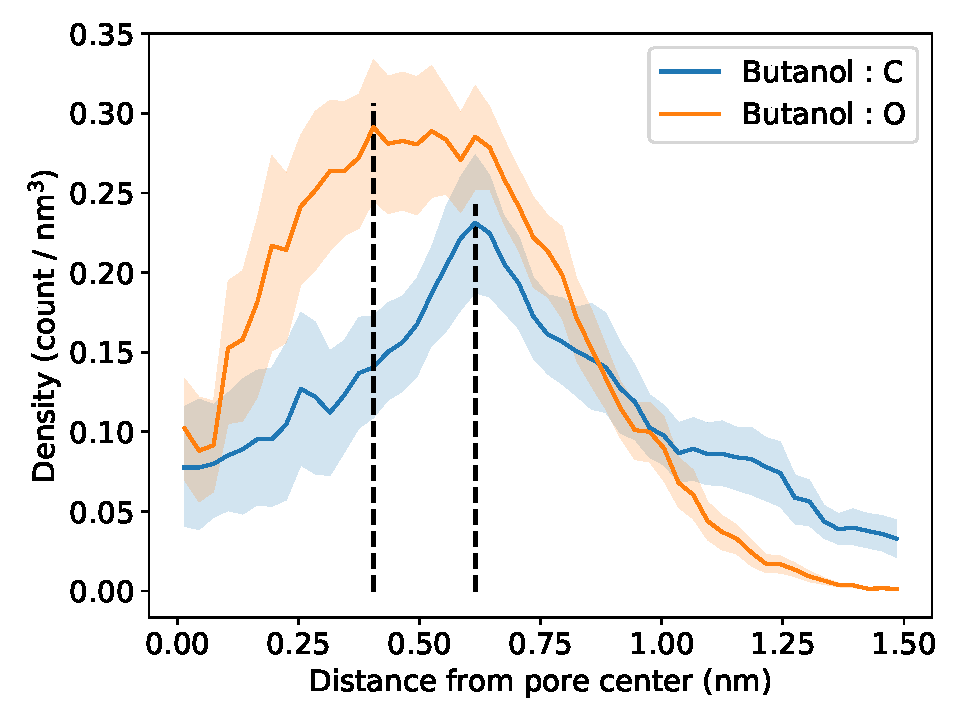
\includegraphics[width=\linewidth]{butanol_CO.pdf}  %BJC: can add inset to plot showing butanol with highlighted O and C
  \caption{}\label{fig:butanol_CO}
  \end{subfigure}
  \caption{(a) The radial distribution functions of each simple alcohol shows a maximum close
  to the highest density of monomer head groups (dashed line, normalized for easier visual
  comparison). Methanol spends the largest proportion of time, relative to the other alcohols,
  near the pore center, which may help explain its fast dynamics. (b) Despite relatively little
  difference in the total number of hydrogen bond occurences, a given alcohol's preference
  towards hydrogen bonds with the carboxylate groups increases with molecule size. (c) The average
  location of butanol's oxygen atom is significantly closer to the pore center than its most distal
  carbon atom, suggesting that the molecule is oriented with hydrophobic tails pointing away from
  the pore center.}\label{fig:simple_alcohols}
  \end{figure}

  \subsection*{Transport of Diols, Triols and Sugars}  % polyols instead of sugars?
  
  Transport is both facilitated and hindered by additional solute hydroxyl groups.
  \begin{itemize}
    \item Extra hydroxyl groups cause solutes to favor the water-rich pore region
    where there is the least hindrance to movement.
    \item However, these extra hydroxyl groups facilitate a larger number of 
    hydrogen bond interactions that work to hold solutes in place.
    \item At the same time, solute molecular weight increases, which inherently
    causes them to move more slowly.
    \item Ethylene glycol, the fastest solute in this grouping (and second fastest
    overall), obtains the best balance of both effects.
  \end{itemize}
  
  The number of hydrogen bonding interactions between solutes and head groups
  increases with the number of solute hydroxyl groups.
  \begin{itemize}
    \item These solutes frequently undergo simultaneous hydrogen bond interactions as
    shown in Figure~\ref{fig:multi_hbonds}. 
    \item For example, both hydroxyl groups of ethylene glycol can undergo hydrogen
    bonds with different hydrogen bond acceptors at the same time.
    \item In some cases, all 4 hydroxyl groups of ribose are hydrogen bonded to monomer
    head groups simultaneously.
%  	\item Simple alcohols, containing only one hydroxyl group, hydrogen bond
%  	with head groups about 20 \% of the time. % BJC: I have a figure showing the average number of hydrogen bonds per solute
  \end{itemize}
  
  \begin{figure}[!htb]
  \centering
  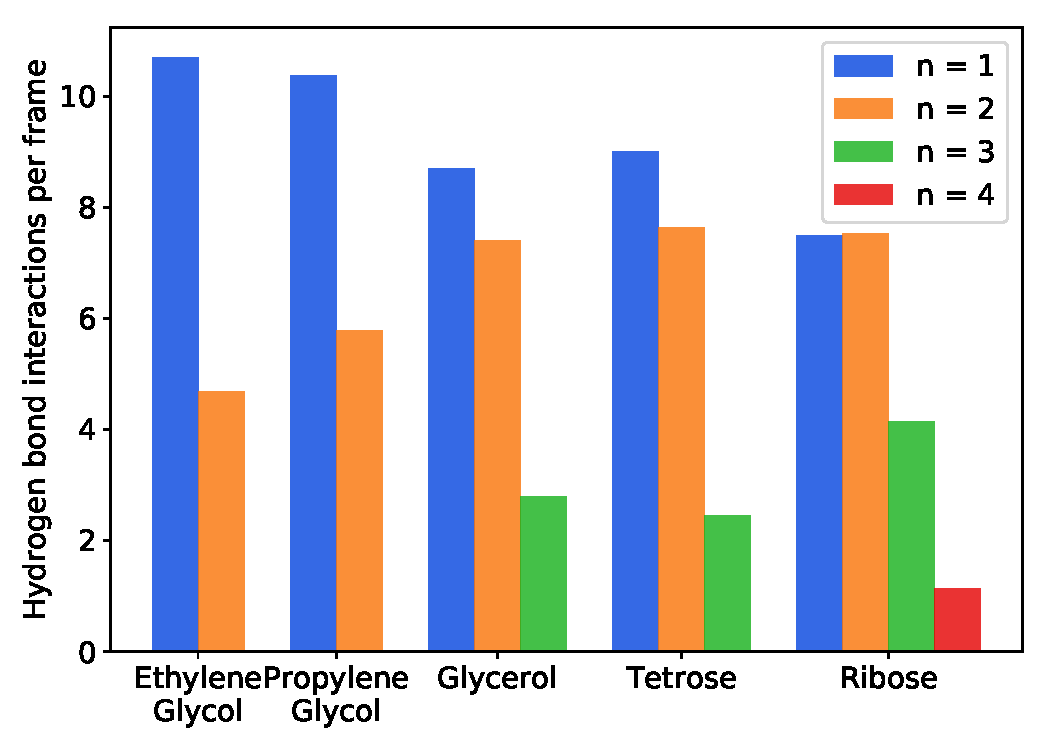
\includegraphics[width=\linewidth]{multi_hbonds.pdf}
  \caption{The number of hydrogen bond interactions between solutes and monomers increases
  as solutes gain additional hydroxyl groups. Multiple hydroxyl groups within a solute often
  hydrogen bond in different locations simultaneously. Occasionally, all four hydroxyl groups
  of Ribose (n = 4) are involved in a hydrogen bond interaction at the same time.}\label{fig:multi_hbonds}
  \end{figure}
  
  Between the two diols, ethylene glycol moves significantly faster than propylene glycol
  due to propylene glycol's affinty for the monomer head groups.  
  \begin{itemize}
  	\item The distribution of each solute's dwell time and hop length distributions shows that
  	ethylene glycol has shorter dwell times and longer hop lengths, which combine to create a 
  	relatively fast MSD. 
    \item Both diols have comparable densities close to the pore center, however propylene glycol's
    density has a large peak near the monomer head groups relative to ethylene glycol. 
    \item Combined with an increase in molecular weight, the addition of a single methyl group
    increases the molecule's hydophobic character and causes propylene glycol to favor positions
    near monomer head groups.
    \item This causes propylene glycol to form more highly stablized hydrogen bonds with
    carboxylate groups, explaining the higher incidence of hydrogen bonds shown in Figure~\ref{fig:multi_hbonds}.
    % BJC: could plot dwell time as a function of radial position (show that dwells are longest when PG
    % is hbonding to head groups
  \end{itemize}
  
  Solutes with three or more hydroxyl groups have the highest density
  at the pore center which contributes to overall faster than expected transport.
  \begin{itemize}
  	\item These molecules are highly water soluble but relatively large
  	\item They can easily hydrogen bond in multiple locations.
  	\item Their large size and high hydrogen bonding capability prevents them
  	from have larger MSDs.
  \end{itemize}
  
  % BJC: Euclidean distance between simultaneous h-bonds for ethylene glycol?
  
%  Ethylene glycol, a diol, has two hydrogen bond donor groups.
%  \begin{itemize}
%	\item Can hydrogen bond with same moeity.
%	\item Can hydrogen bond with different moeities in the same 
%	vicinity. 
%	\item Dwell times tend to be shorter. If one hydroxyl group is bound
%	with a hydrogen bond, the other unbound hydroxyl group may form a hydrogen bond
%	elsewhere and effectively pull the other bound hydroxyl group along with it. 
%  \end{itemize}

  \subsection*{Transport of Thiols} % BJC: maybe put this after next section and call it sulfur analogs and include DMSO?
  
  We studied the transport properties of sulfur analogs of glycerol and ethylene glycol.
  \begin{itemize}
    \item We replaced all but one oxygen atom of each solute with sulfur atoms
  	\item Sulfur is unable to hydrogen bond, however it is soluble in water  %BJC: maybe a reference to why sulfur can't hbond
  	\item Comparisons of their RDFs are shown in Figure~\ref{fig:sulfur_analog_rdfs}.
  \end{itemize}
  
  \begin{figure}
  \centering
  \begin{subfigure}{0.45\linewidth}
  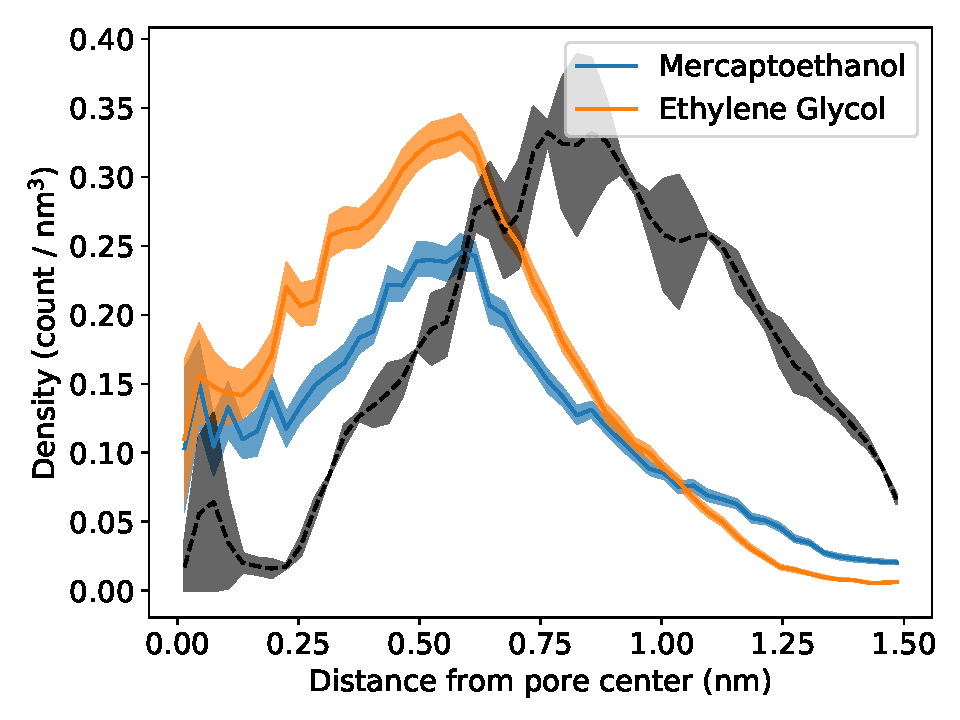
\includegraphics[width=\textwidth]{thiol_comparison_SOH.pdf}
  \caption{}\label{fig:SOH_GCL_comparison}
  \end{subfigure}
  \begin{subfigure}{0.45\linewidth}
  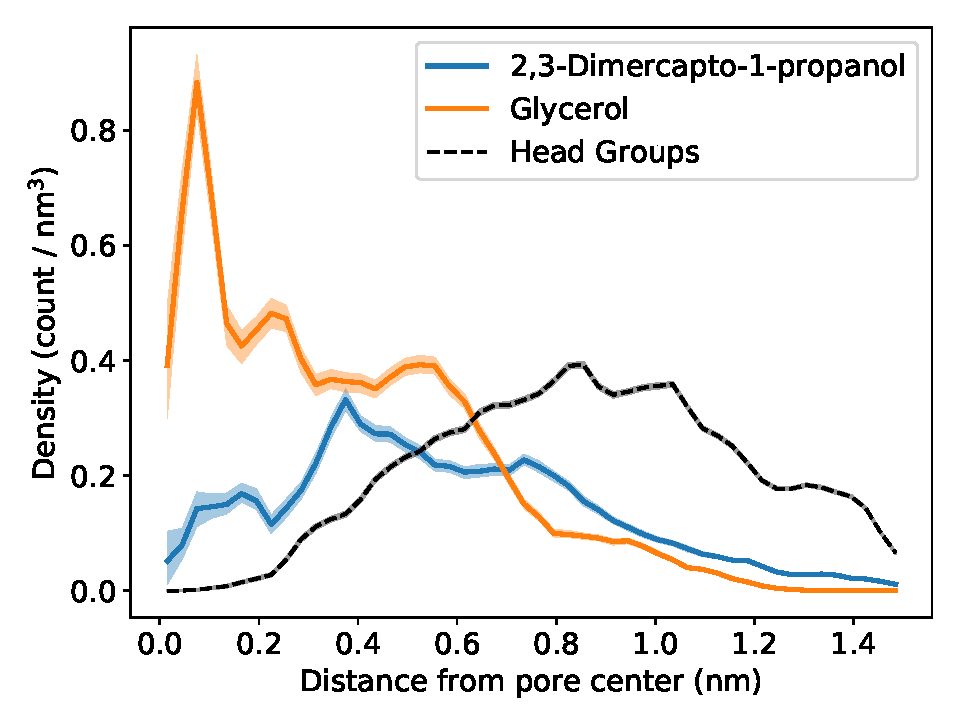
\includegraphics[width=\textwidth]{thiol_comparison_DMP.pdf}
  \caption{}\label{fig:DMP_GLY_comparison}
  \end{subfigure}
  \caption{}\label{fig:sulfur_analog_rdfs}
  \end{figure}
  
  \noindent Mercaptoethanol has a similar average RDF and MSD to ethylene glycol.
  \begin{itemize}
    \item There is a much larger uncertainty associated with mercaptoethanol's MSD
    % BJC: hypothesis about observation. Remains to be quantified
    \item Mercaptoethanol exhibits some of the largest single observed hops among all solutes.
    \item Less frequent hydrogen bonding and an affinity for the pore region may be responsible
    for these hops.
  \end{itemize}
  
  \noindent 2,3-Dimercapto-1-propanol exhibits slower transport than glycerol because it spends more time
  near monomer head groups. %BJC: should I give all the solutes nicknames (i.e. their residue names)?
  \begin{itemize}
    \item Glycerol frequently hydrogen bonds with more than one head group at a time.
    \item It also hydrogen bond with water molecules which causes it to stay in the pore region
    \item 2-3-Dimercapto-1-propanol preferentially hydrogen bonds with head groups so it stays
    close to pore walls.
  \end{itemize} 

  \subsection*{Transport of Ketones}
  
  %BJC: DMSO might be added to this section. 
  %BJC: DMSO might be slow because it's miscible in organic and polar solvents  
  
  The 4 ketone-like molecules tested show a range of transport behaviors.
  \begin{itemize}
    \item Urea, Acetic Acid, Acetamide and Acetone are all characterized by a carbonyl group
    with two attached heavy atoms. 
    \item All have approximately the same molecular weight and are planar molecules due to
    the sp2 hybridization of the carbonyl group.
    \item The fastest solute of this grouping, Urea, has an MSD comparable to that of ethylene
    glycol while the slowest, Acetone, has an MSD one third of that of Urea.
  \end{itemize}
  
  Once again, the trends in the MSD can in large part be explained by the solutes'
  ability to hydrogen bond.  % or maybe just polarity
  \begin{itemize}
  	\item Urea, Acetic Acid and Acetamide are all capable of donating hydrogen bonds,
  	while acetone is the first instance of a molecule in this study that can only
  	accept hydrogen bonds.
  	\item Urea has two hydrogen bond donor nitrogen atoms. It is not surprising that
  	its density is high near the pore center, particularly near the monomer head groups.
  	\item Acetamide has only one nitrogen atom. One of two peaks in its density is 
  	located close to the peak of Urea, likely corresponding to hydrogen bonds with head groups.
  	A second peak is located within the head group region. %BJC: hbonds with ethers vs. head groups. Or is it just planarity?
  	\item Acetic acid, a carboxylic acid shows a relatively high density in the pore region, with 
  	a peak close to the carboxylate groups.  %BJC: hbonds with 
  	\item Acetone is stabilized by accepting hydrogen bonds from water in the pore region, but
    its low polarity and planar shape gives it comparable stability when trapped between head groups.
%  	\item Acetone's has two prominent peaks in its radial density. One is in the pore region and the o
%  	other is relatively deep in the head group region.
  \end{itemize}
  
  \subsection*{Hydrogen bond acceptors}  % Need a better heading since all molecules in this study are acceptors
  
  The final set of molecules we studied can accept hydrogen bonds, but cannot donate
  them. 
  \begin{itemize}
  	\item Among this set are the two slowest solutes in our study: Tetrahydrofuran and Dimethyl Formamide.
  	\item Ethyl acetate and Propylene Carbonate are only marginally faster, however they
  	are both larger molecules. %BJC: not sure how far I should dive into this point
  \end{itemize}
  
  The radial density functions highlight the solutes' preference for the 
  pore region.
  \begin{itemize}
  	\item There are small peaks in the radial density greater than 1 nm 
  	from the pore center.
  	\item The solutes become trapped in these regions where each step is
  	highly anti-correlated to its previous step, leading to very low MSDs.
  	\item The large size and nonplanar shapes of ethyl acetate and propylene 
  	carbonate may destabilize entrapment in the tail region more quickly, leading
  	to slightly faster transport. 
%  	\item The relatively small amount of movement on the timescales studied 
%  	do not reveal definitive reasons
  	\item Overall, 
  \end{itemize}
  Ethyl acetate spends all of its time in a linear or near-linear conformation. % can show with dihedrals
  
  THF and DMF are both planar which allows them to 
  

  % THF shows highly anticorrelated hops
  
  %All have comparable densities near pore center except acetone which is lower

%  \subsection*{Transport of Ions} % probably just sodium
%
%  Sodium ions also exhibit hop diffusion because polarized water and
%  carboxylate head groups both work to neutralize its charge.
%  \begin{itemize}
%	\item Ions get trapped in oxygen 'cages' composed of combinations
%	of water molecules, carboxylate head groups and ether oxygens connecting
%	the head groups to their tails.
%  	\item Interesting coordination number data
%	\item Dwell time proportional to surrounding charge within coordination shell
%  \end{itemize}

  \subsection{Design Principles}

  Water content affects pore size. Experiments to understand this could be useful.

  Separate polar molecules by creating monomers with more hydrophilic head group components.
  More incentive to dwell on walls.

  Make ions move faster by placing charges in sterically inaccessible places. 

  \section{Conclusion}

  We have examined the transport characteristics of a series of small polar
  molecules in our model of the H\textsubscript{II} phase formed by 
  Na-GA3C11.

  We calculated the macroscopic diffusion coefficients of each solute as 
  approximated by a CTRW model and validated our estimates using experimental
  DOSY NMR measurements.

  We have studied the influence of water content on the diffusion coefficients.

  We showed that hydrogen bonding between solutes and Na-GA3C11 monomers plays
  a major role in mechanism by which molecules traverse the nanopores. 

  We can use this intuition in order to modify our monomers for a specific 
  separation.
  \begin{itemize}
	\item Increase number of h-bond sites to increase selectivity towards water 
	over polar molecules
	\item Also separate acetone (things with only h-bond accepting groups) in this way
  \end{itemize}
  
 
  \section*{Supporting Information}

  Detailed explanations and expansions upon the results and procedures mentioned in
  the main text are described in the Supporting Information. This information is
  available free of charge via the Internet at http://pubs.acs.org.

  \section*{Acknowledgements}

  Molecular simulations were performed using the Extreme Science and
  Engineering Discovery Environment (XSEDE), which is supported by National
  Science Foundation grant number ACI-1548562. Specifically, it used the Bridges
  system, which is supported by NSF award number ACI-1445606, at the Pittsburgh
  Supercomputing Center (PSC). This work also utilized the RMACC Summit supercomputer,
  which is supported by the National Science Foundation (awards ACI-1532235 and
  ACI-1532236), the University of Colorado Boulder, and Colorado State
  University. The Summit supercomputer is a joint effort of the University of
  Colorado Boulder and Colorado State University.

  \clearpage

  \bibliographystyle{ieeetr}
  \bibliography{transport}

  \newpage

  \section*{TOC Graphic}

\end{document}
